\definecolor{zzttqq}{rgb}{0.6,0.2,0.}
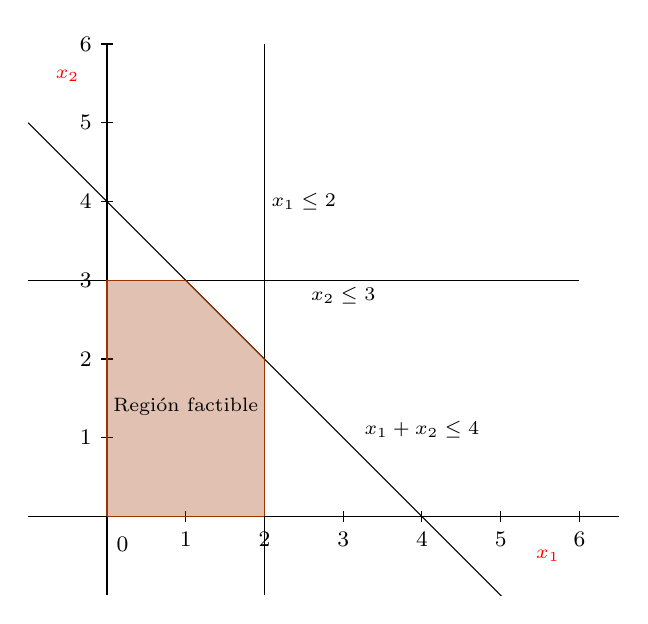
\begin{tikzpicture}[x=1.0cm,y=1.0cm]
\draw[color=black] (-1,0) -- (6.5,0);
\foreach \x in {1,2,3,4,5,6}
\draw[shift={(\x,0)},color=black] (0pt,2pt) -- (0pt,-2pt) node[below] {\footnotesize $\x$};
\draw[color=black] (0,-1) -- (0.,6);
\foreach \y in {1,2,3,4,5,6}
\draw[shift={(0,\y)},color=black] (2pt,0pt) -- (-2pt,0pt) node[left] {\footnotesize $\y$};
\draw[color=black] (0pt,-10pt) node[right] {\footnotesize $0$};
\clip(-1.,-1.) rectangle (6.,6.);
\fill[color=zzttqq,fill=zzttqq,fill opacity=0.30000001192092896] (0.,3.) -- (1.,3.) -- (2.,2.) -- (2.,0.) -- (0.,0.) -- cycle;
\draw [domain=-1.:6] plot(\x,{(--3.-0.*\x)/1.});
\draw (2.,-1.) -- (2.,7.);
\draw [domain=-1.:6] plot(\x,{(--4.-1.*\x)/1.});
\draw [color=zzttqq] (0.,3.)-- (1.,3.);
\draw [color=zzttqq] (1.,3.)-- (2.,2.);
\draw [color=zzttqq] (2.,2.)-- (2.,0.);
\draw [color=zzttqq] (2.,0.)-- (0.,0.);
\draw [color=zzttqq] (0.,0.)-- (0.,3.);
\begin{scriptsize}
\draw[color=black] (3,2.8) node {$x_2\leq 3$};
\draw[color=black] (2.5,4) node {$x_1 \leq 2$};
\draw[color=black] (4.0,1.1) node {$x_1+x_2 \leq 4$};
\draw[color=black] (1,1.4) node {$\mathrm{Regi\acute{o}n\ factible}$};
\draw[color=red] (5.6, -0.5) node {$x_1$};
\draw[color=red] (-0.5,5.6) node {$x_2$};
\end{scriptsize}
\end{tikzpicture}